\documentclass[a4paper, 11pt]{report}

\usepackage[margin=1in]{geometry}

\usepackage[hidelinks]{hyperref}

\usepackage{enumitem}


\usepackage[utf8]{inputenc}
\usepackage[english,greek]{babel}
%\usepackage[LGR]{fontenc}

%\renewcommand{\familydefault}{\sfdefault}



\usepackage{graphicx}
\graphicspath{ {images/} }

\usepackage[usenames, dvipsnames]{color}
\definecolor{mygray}{gray}{0.6}

%make pdflatex output copy-and-paste-able
\input{glyphtounicode}
\pdfgentounicode=1

%shortcuts
\newcommand{\gr}{\selectlanguage{greek}}
\newcommand{\en}{\selectlanguage{english}}

\definecolor{calpolypomonagreen}{rgb}{0.07, 0.53, 0.03}


\usepackage{listings}

\lstdefinelanguage{diff}{
  morecomment=[f][\color{blue}]{@@},     % group identifier
  morecomment=[f][\color{red}]-,         % deleted lines 
  morecomment=[f][\color{calpolypomonagreen}]+,       % added lines
  morecomment=[f][\color{magenta}]{---}, % Diff header lines (must appear after +,-)
  morecomment=[f][\color{magenta}]{+++},
}

\lstdefinelanguage{diffrrr}{
  sensitive=true,
  % diff command line
  morecomment=[f][\color{gray}][0]{diff},
  % commit identifiers for git diff
  morecomment=[f][\color{gray}][0]{index},
  % hunk location/line numbers for unified format
  morecomment=[f][\color{blue}][0]{@@},
  % hunk location/line numbers for context format
  morecomment=[f][\color{magenta}][0]{***},
  % changed line for context format
  morecomment=[f][\color{violet}][0]{!},
  % deleted lines for unified format
  morecomment=[f][\color{red!60!black}][0]-,
  % added lines for unified format
  morecomment=[f][\color{green!60!black}][0]+,
  % file name and time stamp old file
  morecomment=[f][\color{magenta}][0]{---},
  % file name and time stamp new file
  morecomment=[f][\color{magenta}][0]{+++},
  % Binary files ... differ
  morecomment=[f][\color{gray}][0]{Binary},
  % Only in ...: file.txt
  morecomment=[f][\color{gray}][0]{Only},
  % old mode ...
  morecomment=[f][\color{gray}][0]{old},
  % new mode ...
  morecomment=[f][\color{gray}][0]{new},
  % rename from/to ...
  morecomment=[f][\color{gray}][0]{rename},
  % similarity index ...%
  morecomment=[f][\color{gray}][0]{similarity},
  % deleted file mode ...%
  morecomment=[f][\color{gray}][0]{deleted},
  % hunk separator for context format
  morecomment=[f][\color{magenta}][0]{***************},
  % deleted lines for normal format
  morecomment=[f][\color{red!60!black}][0]<,
  % added lines for normal format
  morecomment=[f][\color{green!60!black}][0]>,
  % line number specifier for normal format
  morecomment=[f][\color{blue}][0]{0},
  % line number specifier for normal format
  morecomment=[f][\color{blue}][0]{1},
  % line number specifier for normal format
  morecomment=[f][\color{blue}][0]{2},
  % line number specifier for normal format
  morecomment=[f][\color{blue}][0]{3},
  % line number specifier for normal format
  morecomment=[f][\color{blue}][0]{4},
  % line number specifier for normal format
  morecomment=[f][\color{blue}][0]{5},
  % line number specifier for normal format
  morecomment=[f][\color{blue}][0]{6},
  % line number specifier for normal format
  morecomment=[f][\color{blue}][0]{7},
  % line number specifier for normal format
  morecomment=[f][\color{blue}][0]{8},
  % line number specifier for normal format
  morecomment=[f][\color{blue}][0]{9},
}[comments]

\definecolor{verbgray}{gray}{0.93}




\lstdefinestyle{myCustomMatlabStyle}{
  language=diff,
  backgroundcolor=\color{verbgray},
  stepnumber=1,
  numbersep=10pt,
  tabsize=4,
  showspaces=false,
  keepspaces=true,
  showstringspaces=false,
  frame=single,
  framerule=0pt,
  columns=fullflexible,
  basicstyle=\ttfamily\footnotesize
}

\lstdefinestyle{myCustomCStyle}{
  language=C,
  backgroundcolor=\color{verbgray},
  stepnumber=1,
  numbersep=10pt,
  tabsize=4,
  showspaces=false,
  showstringspaces=false,
  frame=single,
  framerule=0pt,
  columns=fullflexible,
  basicstyle=\ttfamily\footnotesize
}

\lstdefinestyle{CStyle}{
    backgroundcolor=\color{verbgray},   
    commentstyle=\color{green},
    keywordstyle=\color{magenta},
    numberstyle=\tiny\color{gray}\ttfamily,
    numbers=left,
    stringstyle=\color{purple},
    basicstyle=\ttfamily\small,
    breakatwhitespace=false,         
    breaklines=true,                 
    captionpos=b,                    
    keepspaces=true,                 
    showspaces=false,                
    showstringspaces=false,
    showtabs=false,                  
    tabsize=4,
    columns=fullflexible,
                keywordstyle=\color{blue}\ttfamily,
                stringstyle=\color{red}\ttfamily,
                commentstyle=\color{calpolypomonagreen}\ttfamily,
                morecomment=[l][\color{magenta}]{\#}
    language=C
}

\lstdefinestyle{bash}{
    backgroundcolor=\color{black},   
    commentstyle=\color{white},
    keywordstyle=\color{white},
    stringstyle=\color{white},
    basicstyle=\ttfamily\color{white}\small,
    breakatwhitespace=false,         
    breaklines=true,                 
    %captionpos=b,                    
    keepspaces=true,                 
    showspaces=false,                
    showstringspaces=false,
    showtabs=false,                  
    tabsize=4,
    linewidth=15cm,
    language=C
    %columns=fullflexible,
}



\begin{document}
\begin{center}{\small ΠΑΝΕΠΙΣΤΗΜΙΟ ΠΑΤΡΩΝ - ΤΜΗΜΑ ΜΗΧΑΝΙΚΩΝ Η/Υ ΚΑΙ ΠΛΗΡΟΦΟΡΙΚΗΣ }	
\end{center}

{\Large \noindent\textbf{Λειτουργικά Συστήματα}
\hfill \textbf{Άσκηση 4}}

\begin{flushright}
	\textbf{Εργασία Φοιτητή:}\\
	Δαμιανός Ντούμη - Σιγάλας, 6157\\
	\texttt{\en \href{mailto:nsigalas@ceid.upatras.gr}{nsigalas@ceid.upatras.gr}\gr}
\end{flushright}

\lstset{basicstyle=\large,style=myCustomMatlabStyle}


\setlength{\parskip}{10pt}%

\vspace{-0.5cm}

\noindent \textbf{{\large Ερώτημα Α}}

\noindent \textbf{Τροποποιηθέν Αρχείo:}
\vspace{-0.2cm}

\noindent \texttt{\en /usr/src/servers/vfs/protect.c\gr}

\en
\lstinputlisting[language=diff]{code/A_hw4.patch}
\gr

\noindent \textbf{\en Screenshot \gr αποτελεσμάτων:}
\vspace{-0.2cm}

\noindent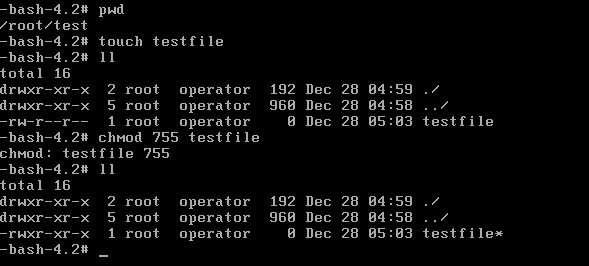
\includegraphics[scale=0.6]{A_patch}


\noindent \textbf{{\large Ερώτημα B}}

\noindent \textbf{Τροποποιηθέν Αρχείo:}
\vspace{-0.2cm}

\noindent \texttt{\en /usr/src/kernel/system/do\_fork.c\gr}

\en
\lstinputlisting[language=diff]{code/B.patch}
\gr

\noindent \textbf{\en Screenshot \gr αποτελεσμάτων:}
\vspace{-0.3cm}

\noindent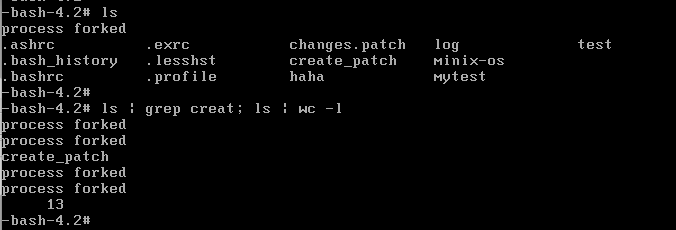
\includegraphics[scale=0.65]{B_patch}

\noindent \textbf{{\large Ερώτημα Γ}}

\noindent \textbf{Τροποποιηθέντα Αρχεία:}

\vspace{-0.65cm}

\en
\begin{enumerate}[itemsep=-1ex,partopsep=1ex,parsep=1ex]
\item \texttt{/usr/src/servers/pm/table.c}
\item \texttt{/usr/src/servers/pm/proto.h}
\item \texttt{/usr/src/include/minix/callnr.h}
\item \texttt{/usr/src/servers/pm/misc.c}
\end{enumerate}
\gr

\en
\lstinputlisting[language=diff]{code/C_table.patch}
\lstinputlisting[language=diff]{code/C_proto.patch}
\lstinputlisting[language=diff]{code/C_callnr.patch}
\lstinputlisting[language=diff]{code/C_misc.patch}

\gr
Για την δοκιμή αυτού του ερωτήματος, υλοποιείται ένα επιπλέον πρόγραμμα σε \en C\gr\footnote{Ο κώδικας των προγραμμάτων που χρησιμοποιήθηκαν για τις δοκιμές, παρατίθεται στο τέλος της αναφοράς.} το οποίο με την χρήση της δημιουργηθείσας κλήσης συστήματος εμφανίζει το πλήθος των διεργασιών που τρέχουν πριν, κατά την διάρκεια και μετά την δημιουργία θυγατρικών διεργασιών. Παρακάτω παρουσιάζονται τα αποτελέσματα για 3 εκτελέσεις του προγράμματος. Παρατηρούμε ότι όταν το πλήθος των διεργασιών που ζητείται ξεπερνά το μέγεθος του \en process table \gr δημιουργούνται τόσες διεργασίες όσες και οι ελεύθερες θέσεις του πίνακα.  

%\begin{center}
   %\noindent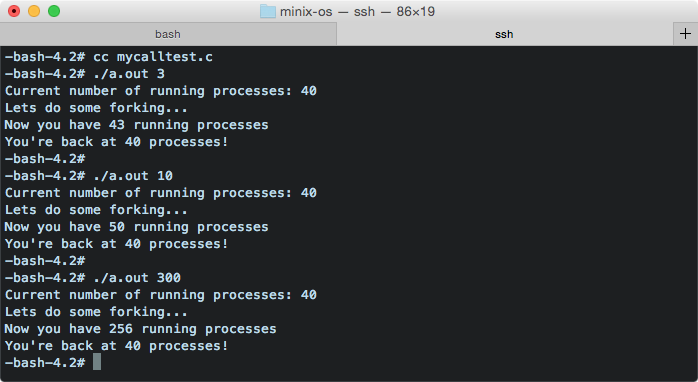
\includegraphics[scale=0.6]{C_test_no.png} 
%\end{center}


\vspace{0.3cm}
\en
\lstinputlisting[style=bash,xleftmargin=1.1cm]{code/C.bash}
\gr


\newpage

\noindent \textbf{{\large Ερώτημα Δ}}

\noindent \textbf{Τροποποιηθέντα Αρχεία:}

\vspace{-0.55cm}

\en
\begin{enumerate}[itemsep=-1ex,partopsep=1ex,parsep=1ex]
\item \texttt{/usr/src/servers/pm/table.c}
\item \texttt{/usr/src/servers/pm/misc.c}
\item \texttt{/usr/src/servers/pm/proto.h}
\item \texttt{/usr/src/include/minix/callnr.h}
\end{enumerate}
\gr

\en
\lstinputlisting[language=diff]{code/D_table.patch}
\lstinputlisting[language=diff]{code/D_misc.patch}

\newpage
\lstinputlisting[language=diff]{code/D_proto.patch}
\lstinputlisting[language=diff]{code/D_callnr.patch}

\gr

Για τον έλεγχο του ερωτήματος αναπτύχθηκε ένα πρόγραμμα σε \en C\gr, το οποίο δίνοντας του ως όρισμα ενα \en pid \gr εκτυπώνει στην οθόνη την τιμή που επιστρέφει η δημιουργηθείσα κλήση συστήματος. Παρακάτω παρουσιάζονται τα αποτελέσματα της εκτέλεσης του.

\vspace{0.3cm}
\en
\lstinputlisting[style=bash,xleftmargin=1.1cm]{code/D.bash}
\gr
\newpage

\noindent \texttt{Δοκιμαστικό πρόγραμμα Γ ερωτήματος}

\lstset{style=CStyle}


\en
\lstinputlisting[language=C]{code/C_test.c}
\gr

\noindent \texttt{Δοκιμαστικό πρόγραμμα Δ ερωτήματος}

\en
\lstinputlisting[language=C]{code/D_test.c}
\gr


\end{document}




%kernel/system/do_fork.c

